
        \documentclass[spanish, 11pt]{exam}

        %These tell TeX which packages to use.
        \usepackage{array,epsfig}
        \usepackage{amsmath, textcomp}
        \usepackage{amsfonts}
        \usepackage{amssymb}
        \usepackage{amsxtra}
        \usepackage{amsthm}
        \usepackage{mathrsfs}
        \usepackage{color}
        \usepackage{multicol, xparse}
        \usepackage{verbatim}


        \usepackage[utf8]{inputenc}
        \usepackage[spanish]{babel}
        \usepackage{eurosym}

        \usepackage{graphicx}
        \graphicspath{{../img/}}



        \printanswers
        \nopointsinmargin
        \pointformat{}

        %Pagination stuff.
        %\setlength{\topmargin}{-.3 in}
        %\setlength{\oddsidemargin}{0in}
        %\setlength{\evensidemargin}{0in}
        %\setlength{\textheight}{9.in}
        %\setlength{\textwidth}{6.5in}
        %\pagestyle{empty}

        \let\multicolmulticols\multicols
        \let\endmulticolmulticols\endmulticols
        \RenewDocumentEnvironment{multicols}{mO{}}
         {%
          \ifnum#1=1
            #2%
          \else % More than 1 column
            \multicolmulticols{#1}[#2]
          \fi
         }
         {%
          \ifnum#1=1
          \else % More than 1 column
            \endmulticolmulticols
          \fi
         }
        \renewcommand{\solutiontitle}{\noindent\textbf{Sol:}\enspace}

        \newcommand{\samedir}{\mathbin{\!/\mkern-5mu/\!}}

        \newcommand{\class}{1º Bachillerato}
        \newcommand{\examdate}{\today}

        \newcommand{\tipo}{A}


        \newcommand{\timelimit}{50 minutos}



        \pagestyle{head}
        \firstpageheader{
\includegraphics[width=0.2\columnwidth]{header_left}}{\textbf{Departamento de Matemáticas\linebreak \class}\linebreak \examnum}{
\includegraphics[width=0.1\columnwidth]{header_right}}
        \runningheader{\class}{\examnum}{Página \thepage\ of \numpages}
        \runningheadrule

        \newcommand{\examnum}{8 - Inecuaciones}
        \begin{document}
        \begin{questions}
        \question p025e01 - Resuelve las inecuaciones lineales:
        \begin{multicols}{2} 
        \begin{parts} \part[1]  $ 5x - 3 \leq 7 - 2x $  \begin{solution}  $ \left(-\infty, \frac{10}{7}\right] $  \end{solution} \part[1]  $ \frac{{2( {x - 3} )}}{5} - \frac{{3x}}{2} + 7 < 10 - \frac{{2x - 3}}{3} $  \begin{solution}  $ \left(-12, \infty\right) $  \end{solution} \part[1]  $ x - 2( {x + 4} ) \leq 3x - 6 $  \begin{solution}  $ \left[- \frac{1}{2}, \infty\right) $  \end{solution} \part[1]  $ \frac{{x - 1}}{2} - \frac{{x + 1}}{3} > 5 - x $  \begin{solution}  $ \left(5, \infty\right) $  \end{solution} \part[1]  $ 2( {x - 6} ) - 5( {x - 4} ) \leq 6x - 1 $  \begin{solution}  $ \left[1, \infty\right) $  \end{solution} \part[1]  $ \frac{{3( {x - 2} )}}{4} - 5( {x + 1} ) > 3 - \frac{x}{4} $  \begin{solution}  $ \left(-\infty, - \frac{19}{8}\right) $  \end{solution} \part[1]  $ 5 - 2( {5x - 6} ) \geq 3( {x - 1} ) + \frac{{7 - x}}{2} $  \begin{solution}  $ \left(-\infty, \frac{33}{25}\right] $  \end{solution} \part[1]  $ 3( {x - 2} ) < 6 $  \begin{solution}  $ \left(-\infty, 4\right) $  \end{solution} \part[1]  $ 2( {x + 3} ) > 3( {x + 2} ) $  \begin{solution}  $ \left(-\infty, 0\right) $  \end{solution} \part[1]  $ 2( {x + 1} ) - 7 \geq x - 3 $  \begin{solution}  $ \left[2, \infty\right) $  \end{solution} \part[1]  $ \frac{{x - 1}}{4} - \frac{{x + 2}}{3} > \frac{{3x - 1}}{6} - x $  \begin{solution}  $ \left(\frac{9}{5}, \infty\right) $  \end{solution} \part[1]  $ \frac{{x - 3}}{5} + \frac{{2x + 6}}{2} \geq \frac{x}{4} - \frac{{3x - 6}}{2} $  \begin{solution}  $ \left[\frac{12}{49}, \infty\right) $  \end{solution} \part[1]  $ {( {x - 3} )^2} - {( {x + 2} )^2} < 5 $  \begin{solution}  $ \left(0, \infty\right) $  \end{solution} \part[1]  $ ( {4x - 3} )( {2 + x} ) > {( {3 - 2x} )^2} $  \begin{solution}  $ \left(\frac{15}{17}, \infty\right) $  \end{solution} \part[1]  $ \frac{{x - 1}}{2} - x < \frac{{1 - x}}{4} - 3 $  \begin{solution}  $ \left(9, \infty\right) $  \end{solution} \part[1]  $ \frac{{x + 7}}{{10}} - \frac{{x - 5}}{5} > \frac{{x - 9}}{3} $  \begin{solution}  $ \left(-\infty, \frac{141}{13}\right) $  \end{solution} \part[1]  $ \frac{{5x - 2}}{3} - \frac{{x - 8}}{4} > \frac{{x + 14}}{2} - 2 $  \begin{solution}  $ \left(4, \infty\right) $  \end{solution} \part[1]  $ 4x - \frac{{3 - 2x}}{4} < \frac{{3x - 1}}{3} + \frac{{37}}{{12}} $  \begin{solution}  $ \left(-\infty, 1\right) $  \end{solution} \part[1]  $ \frac{{x + 2}}{3} - \frac{{12 - x}}{2} > \frac{{5x - 36}}{4} - 1 $  \begin{solution}  $ \left(-\infty, \frac{56}{5}\right) $  \end{solution} \part[1]  $ 3( {x - 2( {\frac{{x - 1}}{4}x - 5} )} ) < \frac{3}{2}( {4 - x} )x $  \begin{solution}  $ \left(20, \infty\right) $  \end{solution} \part[1]  $ \frac{{3x + 1}}{4} - \frac{1}{3} \leq \frac{2}{{15}}( {3x + 2} ) + \frac{{4( {1 - x} )}}{3} $  \begin{solution}  $ \left(-\infty, 1\right] $  \end{solution}
        \end{parts}
        \end{multicols}
        \question p025e02-e04 - Resuelve mediante expresiones algebraicas:
        \begin{multicols}{1} 
        \begin{parts} \part[1] Mezclamos café de 6 euros el kg. con otro de 7,2 euros el kg. y queremos obtener una mezcla de calidad 
    intermedia cuyo precio no pase de 7 euros el kg. para conseguir 60 kg. de esa calidad intermedia, 
    ¿qué condiciones deberán cumplir los pesos de las dos clases mezcladas?  \begin{solution}  $ 6x+7.2(60-x)<7\cdot60  \rightarrow  \\\left(10.0, \infty\right) $  \end{solution} \part[1] Para fabricar un tipo de tapones se tienen como gastos fijos 25 euros de alquiler por la maquinaria y 
    200 de gastos de local. Por otro lado, se calcula que cada tapón supone un gasto de 25 céntimos de euro. 
    Si se dispone de una cantidad de dinero no superior a 1.200 euros, 
    ¿qué número de tapones se puede fabricar si la producción resulta rentable a partir de 3.000 tapones?  \begin{solution}  $ 25+200+0.25x<1200  \rightarrow  \\\left(-\infty, 3900.0\right) $  \end{solution} \part[1] Un padre tiene 32 años más que su hijo, y el abuelo tiene 32 años más que el padre. 
    Hace tres años sus edades sumaban menos de 100 años. 
    ¿Qué edades tienen ahora?. Indica todas las soluciones sabiendo que tienen que ser enteras.  \begin{solution}  $ (x-3-32)+(x-3)+(x-3+32)<100  \rightarrow  \\\left(-\infty, \frac{109}{3}\right) $  \end{solution}
        \end{parts}
        \end{multicols}
        \question p025e05 - Resuelve las inecuaciones:
        \begin{multicols}{2} 
        \begin{parts} \part[1]  $ ( {x - 1} )( {x + 2} )( {x - 3} ) \geq 0 $  \begin{solution}  $ \left[-2, 1\right] \cup \left[3, \infty\right) $  \end{solution} \part[1]  $ \frac{{x - 1}}{{x + 2}} \geq 0 $  \begin{solution}  $ \left(-\infty, -2\right) \cup \left[1, \infty\right) $  \end{solution} \part[1]  $ \frac{{x + 1}}{{x + 3}} < 2 $  \begin{solution}  $ \left(-\infty, -5\right) \cup \left(-3, \infty\right) $  \end{solution} \part[1]  $ ( {x - 2} )( {x + 5} ) > 0 $  \begin{solution}  $ \left(-\infty, -5\right) \cup \left(2, \infty\right) $  \end{solution} \part[1]  $ ( {3x - 5} )( {x + 1} ) \geq 0 $  \begin{solution}  $ \left(-\infty, -1\right] \cup \left[\frac{5}{3}, \infty\right) $  \end{solution} \part[1]  $ 3( {x - 1} )( {x + 2} )( {x + 1} ) \leq 0 $  \begin{solution}  $ \left(-\infty, -2\right] \cup \left[-1, 1\right] $  \end{solution} \part[1]  $ \frac{{x - 2}}{{x + 3}} \leq 0 $  \begin{solution}  $ \left(-3, 2\right] $  \end{solution} \part[1]  $ \frac{{x + 1}}{{x + 2}} > 0 $  \begin{solution}  $ \left(-\infty, -2\right) \cup \left(-1, \infty\right) $  \end{solution} \part[1]  $ \frac{{x - 3}}{{x - 1}} < 5 $  \begin{solution}  $ \left(-\infty, \frac{1}{2}\right) \cup \left(1, \infty\right) $  \end{solution} \part[1]  $ ( {x + 5} )( {x + 2} ) > 0 $  \begin{solution}  $ \left(-\infty, -5\right) \cup \left(-2, \infty\right) $  \end{solution} \part[1]  $ ( {2x - 3} )( {x - 9} ) \leq 0 $  \begin{solution}  $ \left[\frac{3}{2}, 9\right] $  \end{solution} \part[1]  $ 1 - \frac{{x + 3}}{{x + 6}} \geq 0 $  \begin{solution}  $ \left(-6, \infty\right) $  \end{solution} \part[1]  $ \frac{{x + 3}}{{x + 2}} \geq 2 - \frac{x}{2} $  \begin{solution}  $ \left(-2, - \sqrt{2}\right] \cup \left[\sqrt{2}, \infty\right) $  \end{solution} \part[1]  $ \frac{{3x - 2}}{{x - 1}} - 1 \geq \frac{{2x - 1}}{{x + 1}} $  \begin{solution}  $ \left(-1, \frac{1}{2}\right] \cup \left(1, \infty\right) $  \end{solution} \part[1]  $ \frac{{{x^3} - 5{x^2} + 2x + 8}}{x} < 0 $  \begin{solution}  $ \left(-1, 0\right) \cup \left(2, 4\right) $  \end{solution}
        \end{parts}
        \end{multicols}
        \question p026e06 - Resuelve las inecuaciones:
        \begin{multicols}{2} 
        \begin{parts} \part[1]  $ 3{x^2} - 5x + 2 \leq 0 $  \begin{solution}  $ \left[\frac{2}{3}, 1\right] $  \end{solution} \part[1]  $ 5 + 2x < 3{x^2} - 3x + 7 $  \begin{solution}  $ \left(-\infty, \frac{2}{3}\right) \cup \left(1, \infty\right) $  \end{solution} \part[1]  $ 5{x^2} + 20x + 20 > 0 $  \begin{solution}  $ \left(-\infty, -2\right) \cup \left(-2, \infty\right) $  \end{solution} \part[1]  $ 5{x^2} + 20x + 20 \geq 0 $  \begin{solution}  $ \left(-\infty, \infty\right) $  \end{solution} \part[1]  $ 5{x^2} + 20x + 20 < 0 $  \begin{solution}  $ \emptyset $  \end{solution} \part[1]  $ 5{x^2} + 20x + 20 \leq 0 $  \begin{solution}  $ \left\{-2\right\} $  \end{solution} \part[1]  $ 7{x^2} - 5x + 9 > 0 $  \begin{solution}  $ \left(-\infty, \infty\right) $  \end{solution} \part[1]  $ {x^2} - 2x - 8 < 0 $  \begin{solution}  $ \left(-2, 4\right) $  \end{solution} \part[1]  $ 2{x^2} + 3x + 2 \leq 0 $  \begin{solution}  $ \emptyset $  \end{solution} \part[1]  $ {x^2} + x - 6 \geq 0 $  \begin{solution}  $ \left(-\infty, -3\right] \cup \left[2, \infty\right) $  \end{solution} \part[1]  $ {x^2} - 6x + 9 > 0 $  \begin{solution}  $ \left(-\infty, 3\right) \cup \left(3, \infty\right) $  \end{solution} \part[1]  $ {x^2} - 6x + 10 > 0 $  \begin{solution}  $ \left(-\infty, \infty\right) $  \end{solution} \part[1]  $ {x^2} + 8x + 7 < 0 $  \begin{solution}  $ \left(-7, -1\right) $  \end{solution} \part[1]  $ {x^2} + 3 > 4x - 1 $  \begin{solution}  $ \left(-\infty, 2\right) \cup \left(2, \infty\right) $  \end{solution} \part[1]  $ {x^2} + 1 > 2x - 3 $  \begin{solution}  $ \left(-\infty, \infty\right) $  \end{solution} \part[1]  $ 5x + 3 \leq 2{x^2} $  \begin{solution}  $ \left(-\infty, - \frac{1}{2}\right] \cup \left[3, \infty\right) $  \end{solution} \part[1]  $  x \cdot (x - 1)  > 2x + 4 $  \begin{solution}  $ \left(-\infty, -1\right) \cup \left(4, \infty\right) $  \end{solution} \part[1]  $ 3 + x < 5 - x\cdot( {x - 2} ) $  \begin{solution}  $ \left(-1, 2\right) $  \end{solution} \part[1]  $ {x^2} + 16 > 2x $  \begin{solution}  $ \left(-\infty, \infty\right) $  \end{solution} \part[1]  $ \frac{{{x^2} - x}}{3} > 3x - 10 $  \begin{solution}  $ \left(-\infty, \infty\right) $  \end{solution} \part[1]  $ x\cdot( {x + 5} ) > 2{x^2} $  \begin{solution}  $ \left(0, 5\right) $  \end{solution} \part[1]  $ \frac{{( {3 + 2x} )( {x - 1} )}}{3} - 1 > \frac{{{{( {x - 1} )}^2}}}{4} - \frac{{1 + x}}{2} $  \begin{solution}  $ \left(-\infty, - \frac{21}{5}\right) \cup \left(1, \infty\right) $  \end{solution} \part[1]  $ 10( {2x - 1} )( {1 - 3x} ) + 5( {1 - 3x} )( {4x - 1} ) < 3( {1 - 4x} )( {5x - 1} ) $  \begin{solution}  $ \left(-\infty, \frac{3}{10}\right) \cup \left(\frac{2}{3}, \infty\right) $  \end{solution}
        \end{parts}
        \end{multicols}
        \question p026e07 - Resuelve los siguientes sistemas de inecuaciones:
        \begin{multicols}{2} 
        \begin{parts} \part[1]  $ \left\{\begin{matrix}3x - 5 \leq 0\\2x + 8 \geq 0\end{matrix}\right. $  \begin{solution}  $ \left[-4, \frac{5}{3}\right] $  \end{solution} \part[1]  $ \left\{\begin{matrix}2x - 3 > x - 2\\ 3x - 7 < x - 1 \end{matrix}\right. $  \begin{solution}  $ \left(1, 3\right) $  \end{solution} \part[1]  $ \left\{\begin{matrix}2x + 3( {x - 1} ) < x + 1\\2( {x + 3} ) > x + 2 \end{matrix}\right. $  \begin{solution}  $ \left(-4, 1\right) $  \end{solution} \part[1]  $ \left\{\begin{matrix}\frac{{x - 1}}{3} - \frac{{x + 3}}{2} \leq x\\ \frac{{4x - 2}}{4} - \frac{{x - 1}}{3} \geq x\end{matrix}\right. $  \begin{solution}  $ \left[- \frac{11}{7}, - \frac{1}{2}\right] $  \end{solution} \part[1]  $ \left\{\begin{matrix}{( {x - 1} )^2} - {( {x + 3} )^2} \leq 0\\x - 3( {x - 1} ) \geq 3 \end{matrix}\right. $  \begin{solution}  $ \left[-1, 0\right] $  \end{solution} \part[1]  $ \left\{\begin{matrix}\frac{{3( {2 - x} )}}{2} - x < \frac{{16}}{5} - \frac{{x + 1}}{5} \\\frac{{x + 4}}{3} - \frac{{x - 5}}{6} > 3 - \frac{{2x - 3}}{{18}}\end{matrix}\right. $  \begin{solution}  $ \left(\frac{18}{5}, \infty\right) $  \end{solution}
        \end{parts}
        \end{multicols}
        \question p026e08 - Resuelve los siguientes sistemas de inecuaciones:
        \begin{multicols}{2} 
        \begin{parts} \part[1]  $ \left\{\begin{matrix}x + y \leq 2 \\ - 2x + y \geq 4\end{matrix}\right. $  \begin{solution}   \\ 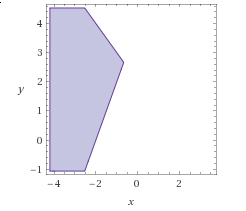
\includegraphics[width=1\columnwidth]{si0}   \end{solution} \part[1]  $ \left\{\begin{matrix}2x - y < 1 \\ - x + 4y \geq  - 5\end{matrix}\right. $  \begin{solution}   \\ 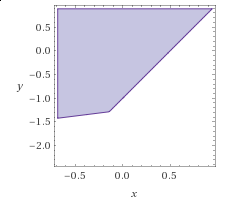
\includegraphics[width=1\columnwidth]{si1}   \end{solution} \part[1]  $ \left\{\begin{matrix}x - 2y > 3\\5x - 3y \leq 15\end{matrix}\right. $  \begin{solution}   \\ 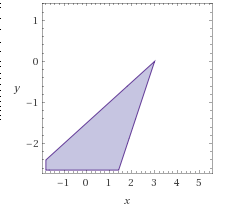
\includegraphics[width=1\columnwidth]{si2}   \end{solution}
        \end{parts}
        \end{multicols}
        
    \end{questions}
    \end{document}
    